\chapter{Verfahrensbeschreibung}\label{ch:verfahrensbeschreibung}


\section{Gesamtsystem}\label{sec:gesamtsystem}
Das System arbeitet nach dem \textbf{EVA}-Prinzip.
Die einzelnen Komponenten laufen jeweils in Threads.
Die \textbf{EVA}-Segmente werden von einem Controller koordiniert, welcher gleichzeitig auch der Einstiegspunkt des Programms ist.
Zu Beginn des Programms nimmt der Controller per Argument einen Ordnerpfad entgegen.
Anschließend startet er die einzelnen Komponenten als Threads.

\subsection{Eingabe}\label{subsec:eingabe}
Sobald er gestartet wurde, liest der Eingabethread permanent Dateien aus dem übergebenen Ordner ein.
Er selbst führt eine Queue, welche alle bereits eingelesenen Dateien enthält.
Alle 0.05s wird von einem weiteren Thread, dessen einzige Aufgabe es ist, eine Methode aufzurufen, ein, nach außen sichtbares, Model ersetzt.
Dadurch wird der gewünschte Effekt simuliert, dass der Detektor mit 20Hz immer eine andere Messreihe zur Verfügung stellt.
Der Controller schaut permanent, ob ein sichtbares Objekt existiert und gibt dieses an die Verarbeitung weiter, falls sich das sichtbare Objekt geändert hat.

\subsection{Verarbeitung}\label{subsec:verarbeitung}
Die Verarbeitungskomponente führt ebenfalls eine Queue, welche von außen befüllt werden kann.
Gibt es ein neues Objekt zum Verarbeiten in der Queue, schaut sie, ob zu diesem Objekt bereits eine Ausgabe existiert.
Ist das nicht der Fall, wird der~\nameref{sec:mathematische-methoden}-Prozess gestartet.
Nach erfolgreicher Berechnung wird das Objekt an die Ausgabeinstanz weitergegeben.

\subsection{Ausgabe}\label{subsec:ausgabe}
Es gibt zwei Ausgabevarianten.
Die eine Ausgabevariante beruht auf der Idee, dass für jeden Schritt (Eingabe, Verarbeitung, Ausgabe) ein einzelner Thread existiert.
Die verarbeitende Instanz befüllt dabei eine Queue des Ausgabethreads, welche von der Ausgabe dann abgearbeitet wird.\\

Die andere Variante ist die, dass die Verarbeitung für jede Messreihe einen einzigen Thread startet.
Dieser ist nach Vollendung seiner Aufgabe, sei es das Schreiben der Datei oder das Ignorieren der Datei, da diese bereits ausgegeben wurde, fertig und läuft nicht in Endlosschleife weiter.\\
Der Vorteil ist zum einen, dass hierfür keine Queue befüllt wird, wodurch Speicherplatz (besonders im Heap) gespart wird und zum anderen die Ausgabe wesentlich schneller verläuft.
Die Ausgabe ist der Teil des Programms, welcher am längsten dauert, wodurch bei dieser Form der Ausgabe der sogenannte \enquote{Bottleneck}-Effekt deutlich verringert wird.
Wurde dieses bisher noch nicht als Datei veröffentlicht, startet dieser Thread den Ausgabeprozess.\\
Bei beiden Varianten wird das berechnete Modell in der vorgegebenen Struktur aus~\autoref{sec:interpretation-der-aufgabe}~in eine~.txt-Datei geschrieben.


\section{Strukturen}\label{subsec:strukturen}
Sowohl die Eingabe als auch die Ausgabe implementieren jeweils ein Interface, welches Runnable erweitert.
Durch das Interface sind implementierende Klassen gezwungen sowohl die Funktion einer Ein-/Ausgabe als auch die eines Runnables zur Verfügung zu stellen.
Runnables sind Objekte, die in einem Thread gestartet werden können.
Dies ermöglicht eine einfache Austauschbarkeit der Komponenten, welche im Controller initialisiert werden.

\subsection{Datenstruktur}\label{subsec:datenstruktur}
Eingelesene Dateien werden in einem Datensatz in einer Liste von Datenpunkten vom Typ Integer gespeichert.
Ein Datenpunkt ist ein generisches Objekt, welches drei Attribute hält.
Diese 3 Attribute sind vom selben Typ, welcher beim Erstellen eines Objekts festgelegt wird.
Im Datenpunkt werden die Position des Spiegels und die Intensität gespeichert.
Nach der Verarbeitung eines Datensatzes enthält dieser eine weitere Liste an Datenpunkten vom Typ Double.
Diese Datenpunkte haben als drittes Attribut zusätzlich den Wert der oberen Einhüllenden befüllt.
Im Datensatz werden außerdem Dateiname, Pulsbreite und das Maximum der Intensität gespeichert.\\
Siehe auch~\nameref{sec:klassendiagramm}.

\protect\pagebreak

\section{Mathematische Methoden}\label{sec:mathematische-methoden}
Nachfolgend werden die in~\nameref{sec:interpretation-der-aufgabe} genannten mathematischen Methoden genauer erläutert, die für den Algorithmus zum Einsatz kommen.

\subsection{Transformierung}\label{subsec:transformierung}
Im ersten Schritt werden die Eingabedaten transformiert.
Dabei wird für jedes eingelesene $\tilde{x}_k \text{ ein } \hat{x}_k$ wie folgt berechnet.
\begin{equation}
    \hat{x}_{k}=\frac{\tilde{x}_{k}}{2^{18}-1} \cdot 266.3-132.3 \quad, \forall k \in[0, N-1]\label{eq:transformation}
\end{equation}
Damit ist $\hat{x}_k$ eine Liste von Pikosekunden.\\
Anschließend wird jedes eingelesene $\tilde{y}_k$ normiert.
Das heißt:
\begin{equation}
    y_k=\frac{\tilde{y}_k}{\tilde{y}_{max}} \quad \text{ mit } \tilde{y}_{max}=\max{\left\{ \tilde{y}_0, \cdots,\tilde{y}_{N-1}\right\}}\label{eq:y_norm}
\end{equation}

\subsection{Glättung}\label{subsec:gleattung}
Auf das Transformieren der x-Werte folgt die Glättung dieser.
Es ist notwendig, da die x-Werte im aktuellen Zustand mit Verzerrungen existieren.
Siehe~\autoref{fig:x_werte_ungeglaettet}.

\begin{figure}[htb]
    \centering
    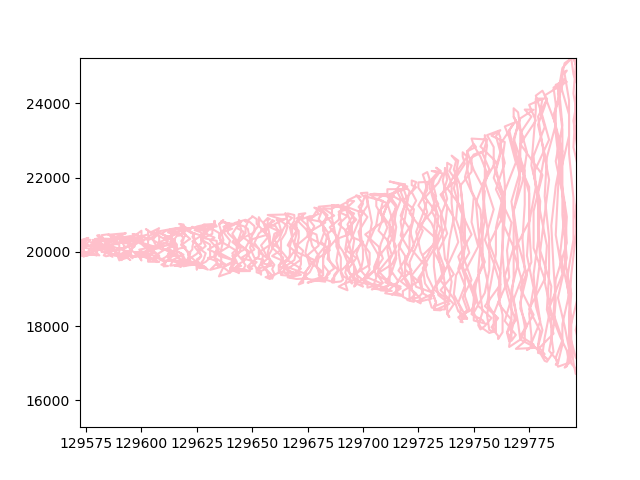
\includegraphics[scale=0.62]{images/Werte_unglatt}
    \caption{Werte ungeglättet und vor Transformation}
    \label{fig:x_werte_ungeglaettet}
\end{figure}

Man berechne hierfür ein $n$ über:

\begin{equation}
    n= \begin{cases}
           \lfloor 0.002 \cdot N\rfloor-1 & , \text { für }\lfloor 0.002 \cdot N\rfloor \text { gerade } \\ \lfloor 0.002 \cdot N\rfloor & , \text { für }\lfloor 0.002 \cdot N\rfloor \text { ungerade }
    \end{cases}\label{eq:auswahl n}
\end{equation}

und jedes $x_k$ dann anschließend über \autoref{eq:glaettung}.
\begin{equation}
    x_{k}=\frac{1}{n} \sum_{i=k-\tau}^{k-\tau+n} \hat{x}_{i} \quad \text { mit } \tau=\frac{n-1}{2}, \forall k \in[0, N-1]\label{eq:glaettung}
\end{equation}
ist $i<0 \text{ oder } i>N-1$ wird der letzt mögliche Wert dupliziert und anstelle von $\hat{x}_{i}$ verwendet.

\begin{align}
    i<0 &: \quad \frac{1}{n}\sum_{i<0} \hat{x}_0\\
    i>N-1 &: \quad \frac{1}{n}\sum_{i>N-1} \hat{x}_{N-1}
\end{align}

Nach dem Glätten sehen die Daten dann aus wie in \autoref{fig:x_werte_glatt}

\begin{figure}[htb]
    \centering
    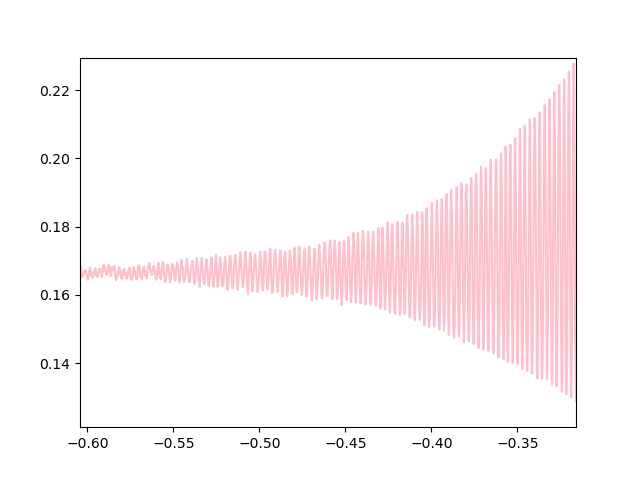
\includegraphics[scale=0.62]{images/Werte_glatt}
    \caption{Werte geglättet und nach Transformation}
    \label{fig:x_werte_glatt}
\end{figure}

\subsection{Wert der oberen Einhüllenden}\label{subsec:wert-der-oberen-einhüllenden}
Für die obere Einhüllende, also der Funktion, welche die lokalen Maximalen y-Werte abbilden soll, muss zuerst das globale Maximum $y_{max}$ bestimmt werden.
Ist dies erfolgt, wird iterativ für jeden Datenpunkt $\{x_k, y_k\}$ bis zum globalen Maximum der bisher höchste Wert als Wert $z_k$ der oberen Einhüllenden gewählt.

\begin{equation}
    z_k= \begin{cases}
             z_{k-1} & , \text { falls } z_{k-1} > y_k \\
             y_k & \text{ sonst }\\
    \end{cases}\label{eq:auswahl_upper_values_left}
\end{equation}
Sobald das globale Maximum erreicht wurde, wird das gleiche Verfahren von rechts wiederholt.
\begin{equation}
    z_k= \begin{cases}
             z_{k+1} & , \text { falls } z_{k+1} > y_k \\
             y_k & \text{ sonst }\\
    \end{cases}\label{eq:auswahl_upper_values_right}
\end{equation}
Wenn auch hier das globale Maximum erreicht wurde, ist die obere Einhüllende berechnet.
$z_k$ wird währenddessen jedem Datenpunkt hinzugefügt

\subsection{Pulsbreite}\label{subsec:pulsbreite}
Für den letzten Schritt des Algorithmus muss die Pulsbreite berechnet werden.
Die Pulsbreite ist die Breite des Signals bei halber Höhe zwischen der Grundlinie und dem Maximum.
Die Grundlinie ist der Mittelwert der ersten $1\% \text{ der } y$-Werte.
Wurde die halbe Höhe berechnet, kann fortgefahren werden.
Es wird wieder von links das Verfahren gestartet und der Datenpunkt gesucht, dessen $z_k \geq h$ ist, wobei $h$ für die halbe Höhe steht.
Der Index $k_l$ dieses Datenpunkts wird zwischengespeichert.
Wird das gleiche Verfahren dann von rechts beginnend wiederholt, kann der Index $k_r$ bestimmt werden.\\
Die Pulsbreite ist dann $x_{k_r} - x_{k_l}$.
Für die Ausgabe werden die Indizes $k_l \text{ und } k_r$ im Datenmodell gespeichert.

\begin{figure}[h]
    \centering
    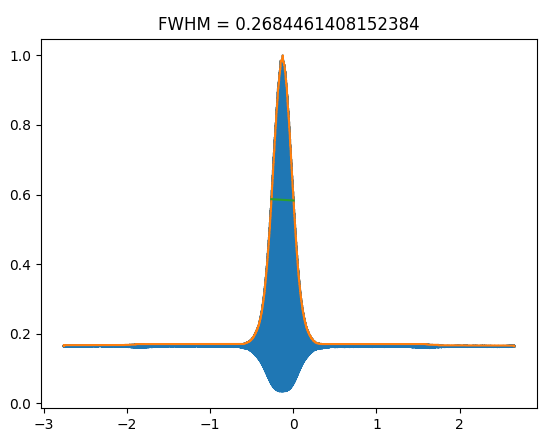
\includegraphics{outFigur}
    \caption{Plot eines ausgegebenen Datensatzes nach seiner Berechnung.
    Der orangene Graph ist die obere Einhüllende, die grüne Gerade die Pulsbreite.
    Durch die Approximation der oberen Einhüllenden, ist diese leicht verzerrt.}
    \label{fig:outplot}
\end{figure}